%----------------------------------------------------------------------------------------
%	PACKAGES AND THEMES
%----------------------------------------------------------------------------------------
\documentclass[aspectratio=169,xcolor=dvipsnames]{beamer}
\usetheme{Simple}

\usepackage{hyperref}
\hypersetup{
    colorlinks,
    linkcolor=black, % Overview
    urlcolor=blue    % \href#2
}

\usepackage{graphicx} % Allows including images

% ding
\usepackage{fancybox}
\usepackage{pifont}
\def\Dstar{\ding{93}}
\def\Dsquare{\ding{114}}
\def\Dok{\ding{52}}
\def\Dko{\ding{56}}
\def\Dhand{\ding{42}}
\def\Dpen{\ding{47}}
\def\Darrow{\ding{220}}

%----------------------------------------------------------------------------------------
%	Macros
%----------------------------------------------------------------------------------------
\newcommand{\bi}{\begin{itemize}}
\newcommand{\ei}{\end{itemize}}
\def\figs{figs1}

%----------------------------------------------------------------------------------------
%	TITLE PAGE
%----------------------------------------------------------------------------------------

% The title
\title[short title]{Introduction to ILDG}

\author{
\includegraphics[scale=0.5]{ildg-logo}\\Hands-on Workshop}
\institute{Francesco Di Renzo - UNIPR \& INFN Parma \\ on behalf of ILDG Board and Working Groups}
\date{June 14, 2023 } % Date, can be changed to a custom date


%----------------------------------------------------------------------------------------
%	PRESENTATION SLIDES
%----------------------------------------------------------------------------------------
\begin{document}

\begin{frame}
    % Print the title page as the first slide
    \titlepage

\end{frame}

\begin{frame}{Overview}
    % Throughout your presentation, if you choose to use \section{} and \subsection{} commands, these will automatically be printed on this slide as an overview of your presentation
    \tableofcontents
\end{frame}

%------------------------------------------------
\section{Motivation and Objectives of ILDG}
%------------------------------------------------
\begin{frame}{Motivation and Objectives of ILDG}
   Gauge configurations in Lattice simulatons are
   \alert{valuable and expensive} in terms of
   \bi
   \item computing resources (i.e. energy, $CO_2$, tax payer's money)
   \item human effort
   \ei

   \vspace*{5mm}
   \begin{block}{Objectives of ILDG}
   \begin{dinglist}{220}
   \item make these precious raw data sharable, usable, and citable for the community
   \item ensure basic quality standards for Lattice data
   \item provide a framework for the organization and putting into
         practice of a solid data management (-plans)
   \end{dinglist}
   \end{block}

   \vspace*{3mm}
   Thus ILDG can and should be beneficial for data consumers \alert{and} data providers!
   
\end{frame}
%------------------------------------------------
\begin{frame}{Caveats}
  
  ILDG is \alert{not} intended as a free solution when running out of disk space

  \vspace*{3mm}
  ILDG does not come for fee, but also \alert{requires effort and resources on users' side}

  \vspace*{3mm}
  On the long run, however, this is likely to pay off, because it can
  \begin{block}{}
  \bi
  \item reduce collaboration-specific efforts for island solutions
  \item increase quality, usability and visibility of Lattice data (and research)
  \item enable funding (and credit) opportunities for essential data management efforts
  \ei
  \end{block}
  
\end{frame}
%================================================
\section{Beginning of ILDG}
%------------------------------------------------
\begin{frame}{Beginning of ILDG}

  \bi
  \item ``Data storage issues in Lattice QCD calculations'' \href{https://arxiv.org/abs/hep-lat/0003009}{C. McNeil 2000}
  \item ILDG proposed by R.D. Kenway in 2002 \\
        ``to manage and exchange lattice data QCD data, particularly gauge configurations''
  \item Concepts presented at Lattice conference in Boston \href{https://arxiv.org/abs/hep-lat/0209121}{2002}
  \item Working Groups for Metadata and Middleware starting in 2002
  \item ILDG Board formed in 2003
  \item Biannual workshops (virtual or at Lattice conferences)
  \item Concise and community-wide agreed \alert{metadata schema} \href{https://arxiv.org/abs/hep-lat/0409055}{2004}
  \item 1st generation of \alert{federated services and infrastructure}\\
        operational in 2007
  \ei

  \vspace*{-30mm}
  \hfill
  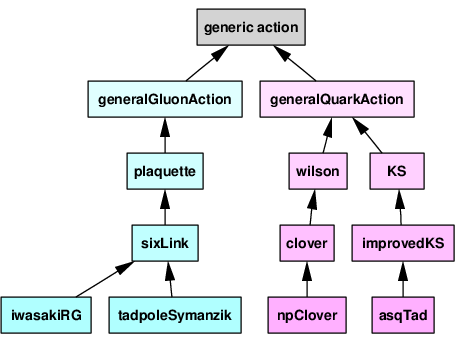
\includegraphics[height=35mm]{\figs/0409055-fig2.png}
  
\end{frame}
%================================================
\section{Basic ILDG Concepts}
%------------------------------------------------
\begin{frame}{Basic Concepts of ILDG}
  \begin{block}{ILDG}
    \begin{itemize}
    \item Federation of \alert{autonomous} ``Regional Grids'' (RG)
    \item Virtual Organisation (VO)
    \item Community-wide agreed standards (QCDml metadata schema, data format, APIs) 
    \end{itemize}
  \end{block}

  \vspace*{5mm}
  {\bf ILDG} operates only \alert{2 global services:}
  \begin{itemize}
  \item VO registration (\href{https://grid-voms.desy.de:8443/voms/ildg}{VOMS}) \\[1mm]
      {\small
        defines VO membership and provides VO-specific authentication attributes
      }
    \item Website (\href{https://hpc.desy.de/ildg}{temporary mirror})\\[1mm]
      {\small 
        specifies standards, services and policies
      }
    \end{itemize}

\end{frame}
%------------------------------------------------
\begin{frame}{Regional Grids}

  \vspace*{3mm}
  \begin{block}{CSSM, JLDG, LDG, UKQCD, USQCD}
    \begin{itemize}
    \item implemented with different architectures and technologies
    \item organized and operated in autonomous ways with individual policies
    \end{itemize}
  \end{block}

  \begin{columns}
    \column{0.4\textwidth}
    % \alert{Each RG} is responsible to provide:
    Responsibility of \alert{each RG} to provide
    \begin{itemize}
    \item Metadata Catalogue (MDC)
    \item File Catalogue (FC)
    \item Storage Elements (SE)
    \item website with RG-specific information
    \end{itemize}

    \column{0.6\textwidth}
    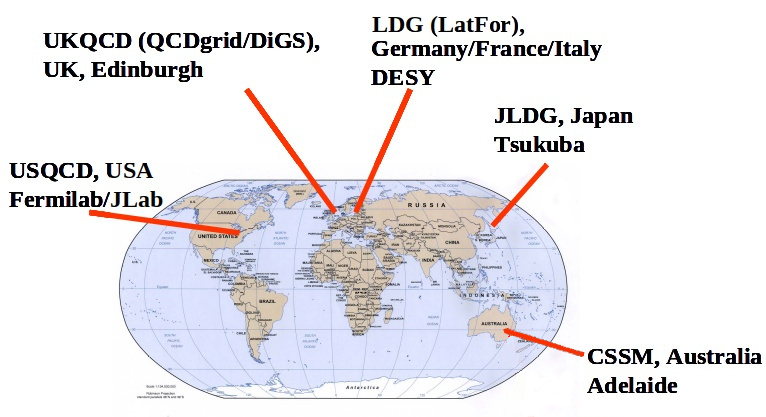
\includegraphics[height=50mm]{\figs/ildg-map-gimp}
  \end{columns}
\end{frame}

%------------------------------------------------
\begin{frame}{Organization of ILDG}
  \begin{dinglist}{114}
    \item {\bf  Board}
    \bi
    \item represents ILDG towards community and service providers
    \item discusses and decides policies and guidelines for membership and data sharing
    \item supports regional grids in applying for resources
    \item oversees working groups
    \ei
  \item {\bf Metadata Working Group (MDWG)} \\
    \bi
    \item agrees on concise and community-wide standards for the description of the data
    \item balances scientific with technical requirements
    \item provides specifications of metadata shema (QCDml) and data formats 
    \ei
  \item {\bf Middleware Working Group (MWWG)} \\
    \bi
    \item specifies interfaces of services to ensure interoperability between all RGs 
    \item supports RGs by exploring technologies and sharing related expertise
    \item suggests or develops prototypes of client tools e.g. for searching and download
    \ei

  \end{dinglist}    

\end{frame}
%------------------------------------------------
\begin{frame}{Pioneering Efforts for ILDG}
  \begin{dinglist}{114}
    \item {\bf  Board} \\
         {\small
           R.~Brower (USA), K.~Jansen (Germany), R.~Kenway (UK), D.~Leinweber (Australia),
           O.~Pene (France), F.~Di~Renzo (Italy), A. Ukawa, T.~Yoshie (Japan)
         }\\[5mm]


       \item {\bf Metadata Working Group (MDWG)} \\
         {\small
           P.~Coddington (Adelaide), T.~Yoshie (Tsukuba), D.~Pleiter (DESY)
           G.~Andronico (INFN), C.~Maynard (Edinburgh), C.~De~Tar (Utah),
           J.~Simone (FNAL), R.~Edwards, B.~Joo (JLAB)
         }\\[5mm]
         
    \item {\bf Middleware Working Group (MWWG)} \\
      {\small
        P.~Coddington, S.~Zang (Adelaide), T.~Amagasa, N.~Ishii, O.~Tatebe, M.~Sato (Tsukuba),
        D.~Melkumyan, D.~Pleiter (DESY), G.~Beckett, R.~Ostrowski (Edinburgh), J.~Simone (FNAL),
        B.~Joo, C.~Watson (JLAB)
      }
  \end{dinglist}
  \hfill   {\small List by T. Yoshie @ HackLatt2009}
\end{frame}


%------------------------------------------------
\begin{frame}{ILDG Middleware in a Nutshell}
  \begin{center}
    \Large{Web services of ILDG (\alert{MDC, FC, SE, VOMS}) implement a\\ \alert{distributed database system} for\\
    \alert{ensemble metadata, configuration metadata, and configuration data}}

  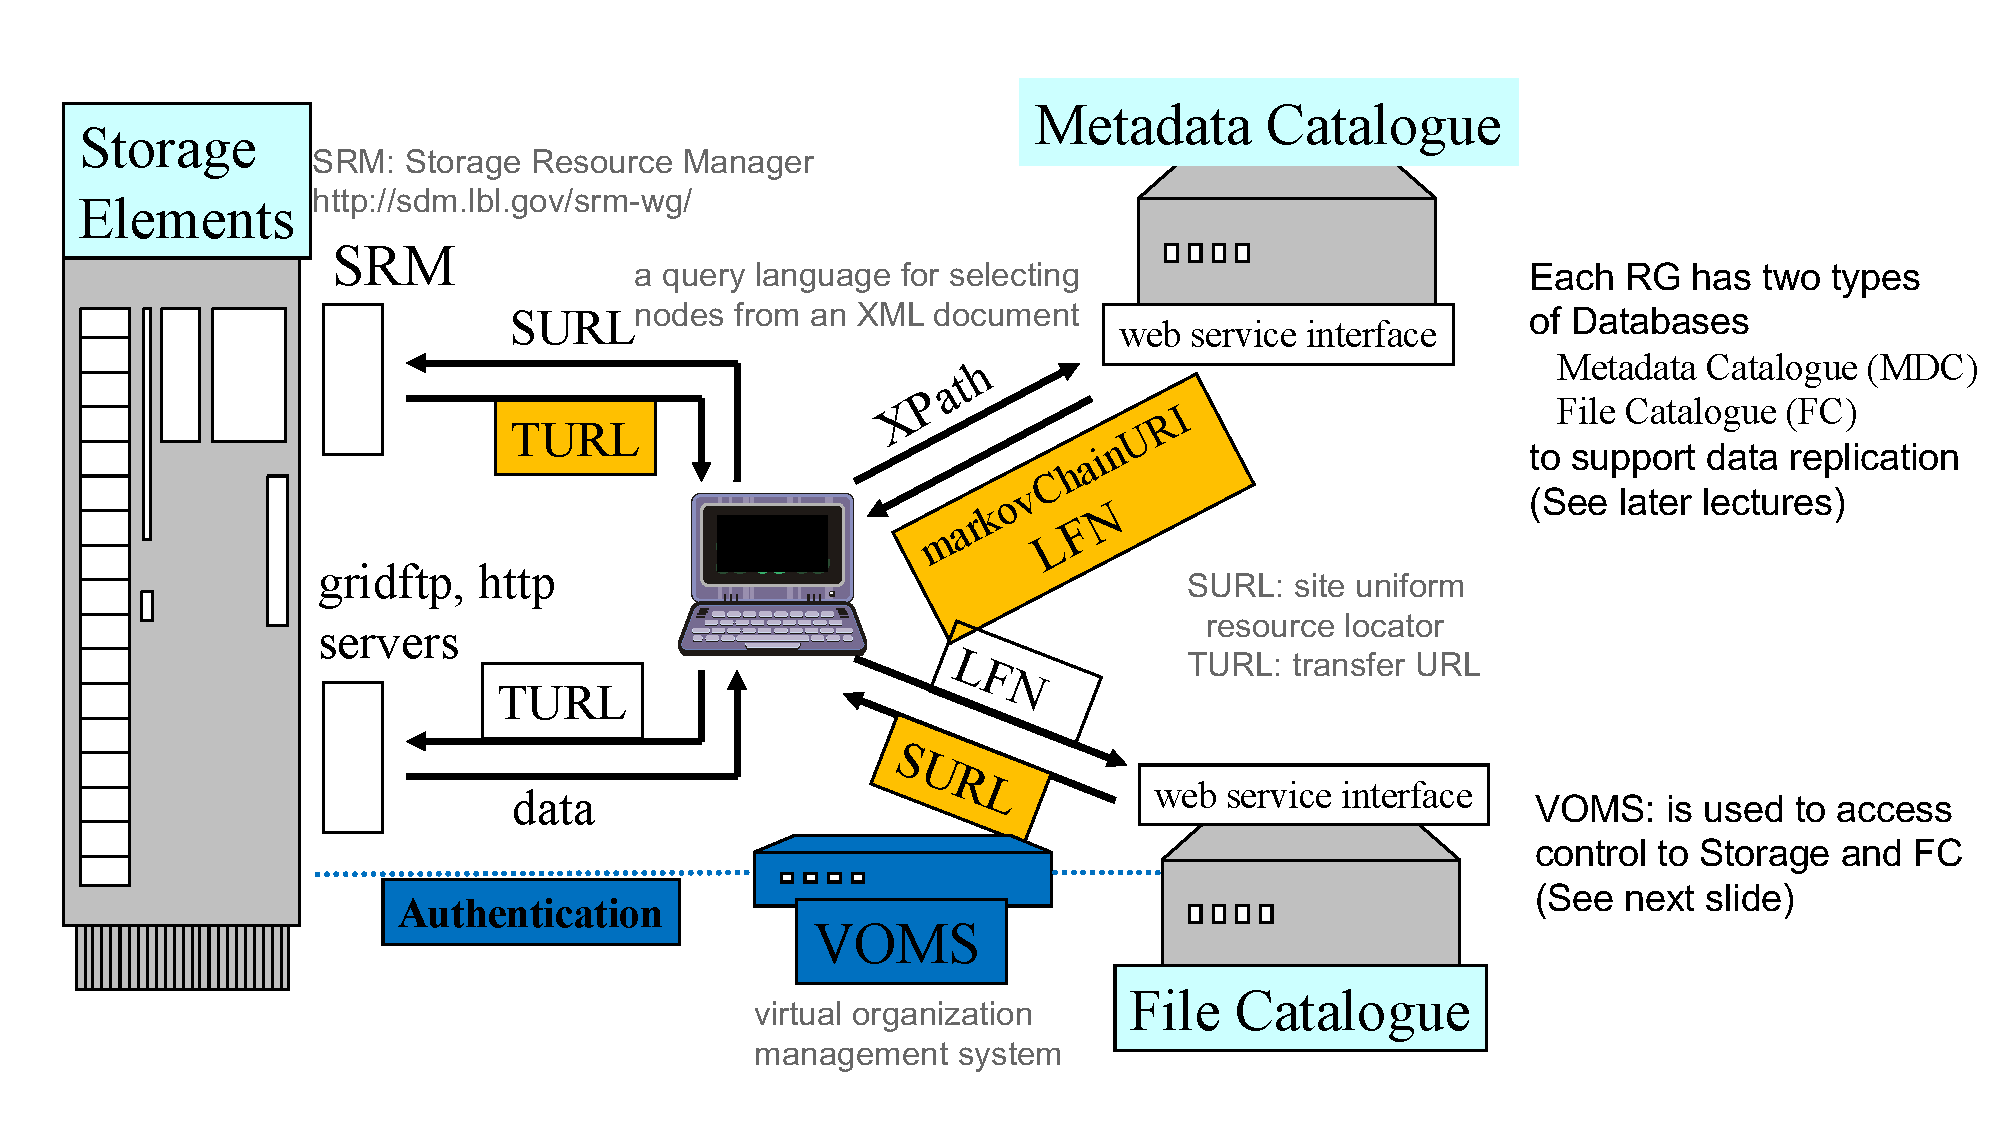
\includegraphics[height=55mm]{\figs/daTY_MW}
  \end{center}

\end{frame}
%------------------------------------------------
\begin{frame}{ILDG Metadata in a Nutshell}

  \begin{center}
    \Large{\alert{QCDml} is a community-agreed, concisely defined, rich and flexible \alert{markup schema},
      which allows \alert{strict validation of metadata}}
    
  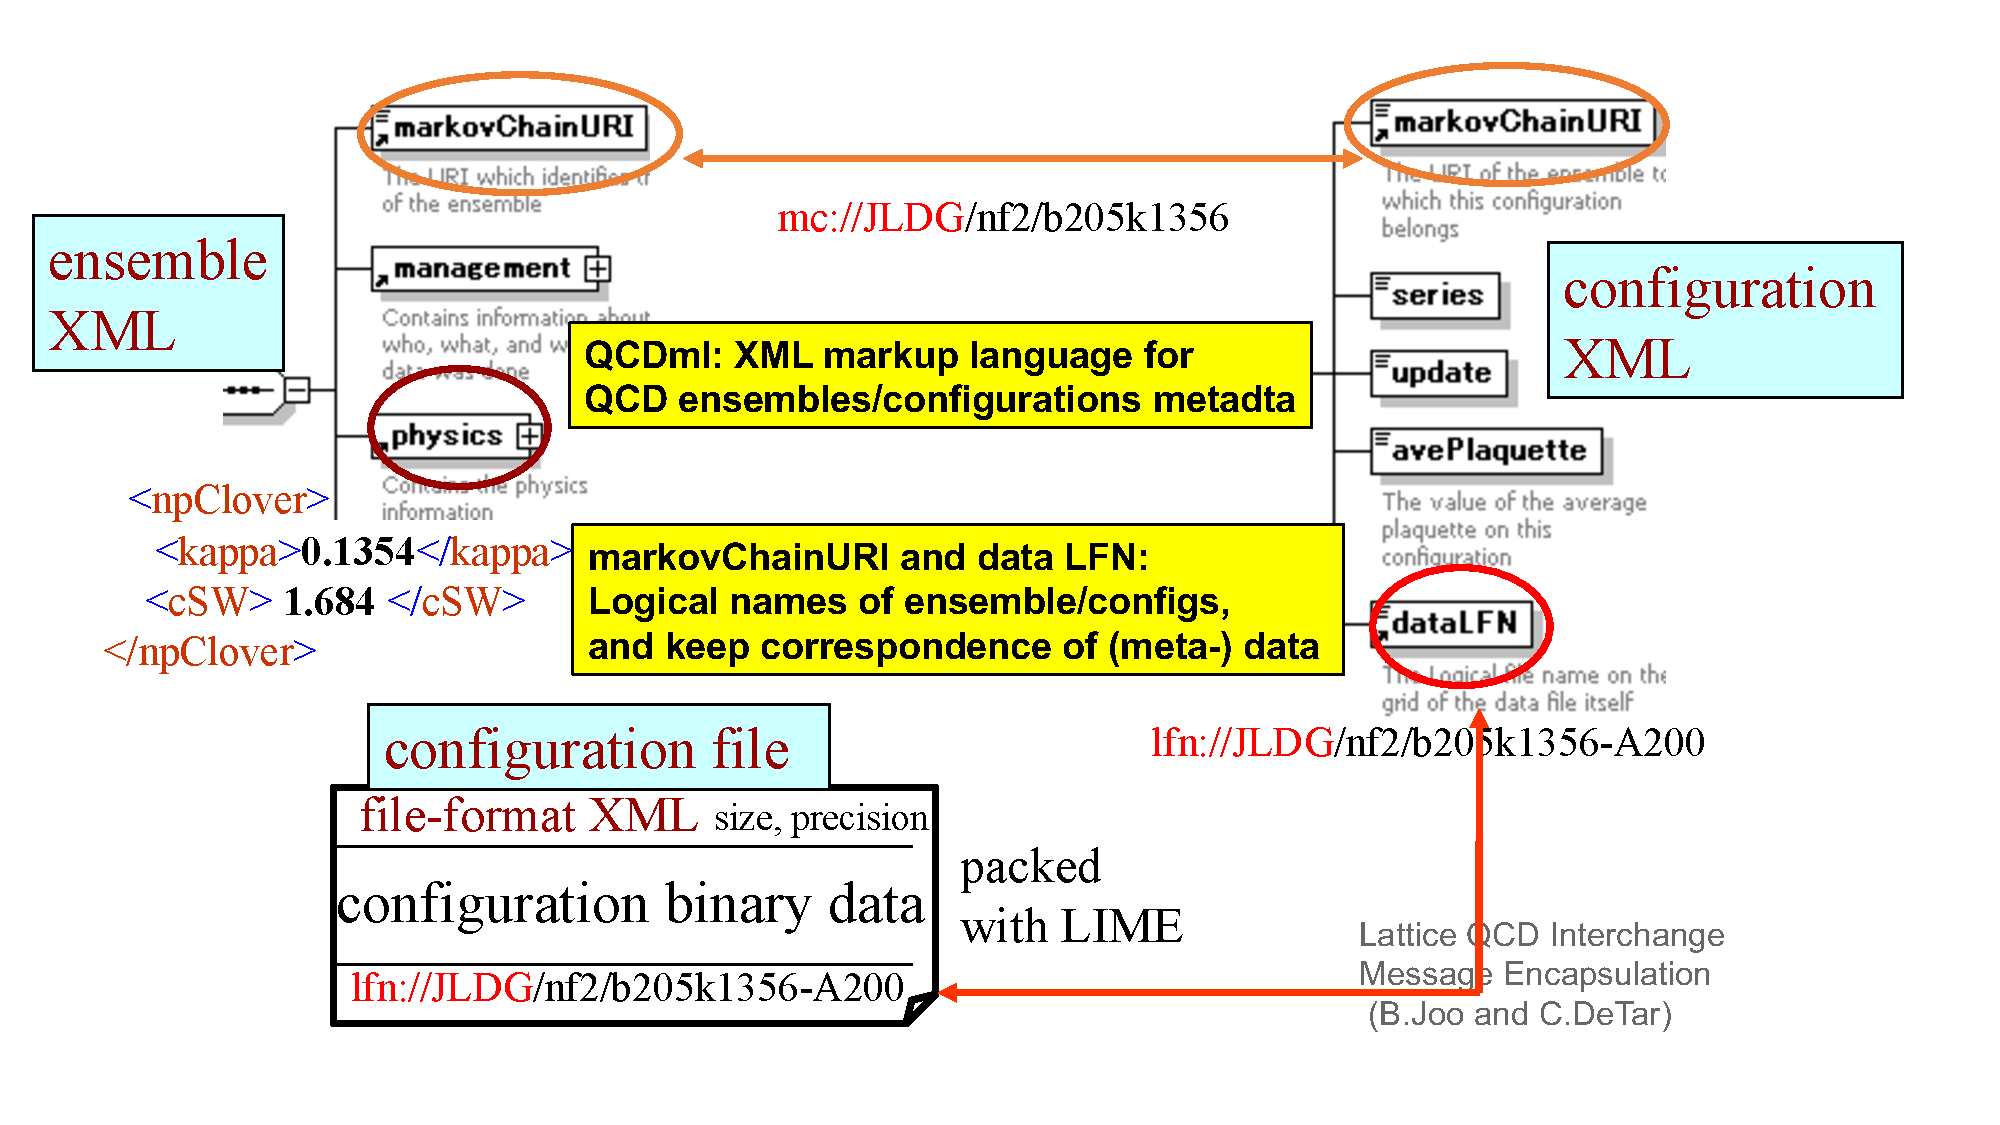
\includegraphics[height=60mm]{\figs/daTY_MD}
  \end{center}
  
\end{frame}
%================================================
\section{Decline and Transition to ILDG 2}
%------------------------------------------------
\begin{frame}{Decline of ILDG}

  During the last 10 years:
  \begin{dinglist}{56}
  \item decreasing (rather than increasing) volume of available storage infrastructure
  \item degrading usability (e.g. client tools only usable by a couple of experts in\\
    those collaborations which continued to heavily use or rely on ILDG)
  \item no alignment with technological develoments (e.g. grid $\to$ cloud) \\
    due to loss of critical person power and expertise
  \item critical services going offline (often because security issues became a serious concern)
  \item no significant activities by Board or Working Groups after 2015
  \end{dinglist}
  Still
  \begin{dinglist}{52}
       \item metadata and data for about 250+59 ensembles (370+30 k configs) \\
       still available in 2 RGs (but accessible only with expert knowledge)
       \item infrastructure still used for data sharing by individual collaborations
\end{dinglist}


\end{frame}
%------------------------------------------------
\section{}
%------------------------------------------------
\begin{frame}{Towards ILDG 2}

  Solid facts to start from
  \begin{dinglist}{52}
     \item pile-up of data from collaborations who want to make configs publicly available\\
     (e.g. $\approx$ 3 PB only in LDG from CLS, ETMC, QCDSF)... AND YOU ARE HERE!
     \item Full implementation of FAIR principles. Research data managment concepts becoming incrisingly important requirement by funding agencies.

  \end{dinglist}

  \hfill  
\includegraphics[height=12mm]{\figs/PUNCH4NFDI-Logo_RGB.jpg}

  \vspace*{-10mm}
  Since 2022:
  \begin{dinglist}{52}
  \item regular Working Group and Board meetings \\
    (current chair: F. Karsch)
  \item dedicated SW developer for re-design of Catalogue Services funded by PUNCH4NFDI\\
    (JLDG+LDG again fully operational, UK RG in preparation)
  \item transition from Grid to Cloud technologies
  \item re-activating communication within and participation by community
    \bi
    \item[\Darrow] Lattice 22 (\href{https://arxiv.org/pdf/2212.08392}{presentation} and
    \href{https://arxiv.org/pdf/2212.10138}{parallel session})
    \item[\Darrow] this Hands-on Workshop
    \ei
  \end{dinglist}
  \vfill
\end{frame}
\section{}
%------------------------------------------------
\begin{frame}{Concluding Remarks}

  \begin{dinglist}{114}

  \item Very diverse perspectives on (and use-cases of) ILDG
    \bi
    \item data consumer vs. data provider
    \item restricted (within or between collaborations) vs. public sharing
    \ei
  \item ILDG is \alert{not} a commercial service
    \bi
    \item can only be realized as community effort
    \item uni-directional propagaton of knowledge and efforts can not work
    \ei
 
  \item ILDG 2 is work in progress
    \bi
    \item still a long way to go
    \item needs replacement of components and adiabatic changes of setup
    \item your feedback and participation is crucial to further develop ILDG
    \ei
  \end{dinglist}
    
\end{frame}
%----------------------------------------------------------------------------------------
\end{document}



